%%%%%%%%%%%%%%%%%%%%%%%%%%%%%%%%%%%%%%%%%%%%%%%%%%%%%%%%%%%%%%%%%%%%%%
% LaTeX Template: Curriculum Vitae 
% Source: http://www.howtotex.com/
%%%%%%%%%%%%%%%%%%%%%%%%%%%%%%%%%%%%%%%%%%%%%%%%%%%%%%%%%%%%%%%%%%%%%%

\documentclass[paper=a4,fontsize=11pt]{scrartcl} % KOMA-article class
							
\usepackage[english]{babel}
\usepackage{graphicx}                    % Enable pdflatex
\usepackage[svgnames]{xcolor}            % Colors by their 'svgnames'
\usepackage{geometry}
	\textheight=650pt
\usepackage{url}
\usepackage{fontawesome}
\usepackage[export]{adjustbox}

\frenchspacing              % Better looking spacings after periods
\pagestyle{empty}           % No pagenumbers/headers/footers

%%% Custom sectioning (sectsty package)
%%% ------------------------------------------------------------
\usepackage{sectsty}

\sectionfont{%			            % Change font of \section command
	\usefont{OT1}{phv}{b}{n}%		% bch-b-n: CharterBT-Bold font
	\sectionrule{0pt}{0pt}{-5pt}{3pt}}

%%% Macros
%%% ------------------------------------------------------------
\newlength{\spacebox}
\settowidth{\spacebox}{8888888888}			% Box to align text
\newcommand{\sepspace}{\vspace*{1em}}		% Vertical space macro

\newcommand{\MyName}[1]{ % Name
		\Huge \usefont{OT1}{phv}{b}{n} \hfill #1
		\par \normalsize \normalfont}
		
\newcommand{\MySlogan}[1]{ % Slogan (optional)
		\large \usefont{OT1}{phv}{m}{n}\hfill \textit{#1}
		\par \normalsize \normalfont}

\newcommand{\NewPart}[1]{\section*{\uppercase{#1}}}

\newcommand{\PersonalEntry}[2]{
		\noindent\hangindent=0em\hangafter=0 % Indentation
		\parbox{\spacebox}{        % Box to align text
		\textit{#1}}		       % Entry name (birth, address, etc.)
		\hspace{2.5em} #2 \par}    % Entry value

\newcommand{\SkillsEntry}[2]{      % Same as \PersonalEntry
		\noindent\hangindent=0em\hangafter=0 % Indentation
		\parbox{\spacebox}{        % Box to align text
		\textit{#1}}			   % Entry name (birth, address, etc.)
		\hspace{2.5em} #2 \par}    % Entry value	

\newcommand{\EducationEntry}[4]{
		\noindent \textbf{#1} \hfill      % Study
		\colorbox{Black}{%
			\parbox{6em}{%
			\hfill\color{White}#2}} \par  % Duration
		\noindent \textit{#3} \par        % School
		\noindent\hangindent=2em\hangafter=0 \small #4 % Description
		\normalsize \par}

\newcommand{\WorkEntry}[4]{				  % Same as \EducationEntry
		\noindent \textbf{#1} \hfill      % Jobname
		\colorbox{Black}{\color{White}#2} \par  % Duration
		\noindent \textit{#3} \par              % Company
		\noindent\hangindent=2em\hangafter=0 \small #4 % Description
		\normalsize \par}

%%% ------------------------------------------------------------
\begin{document}

\begin{figure}
    \vspace*{60pt}
    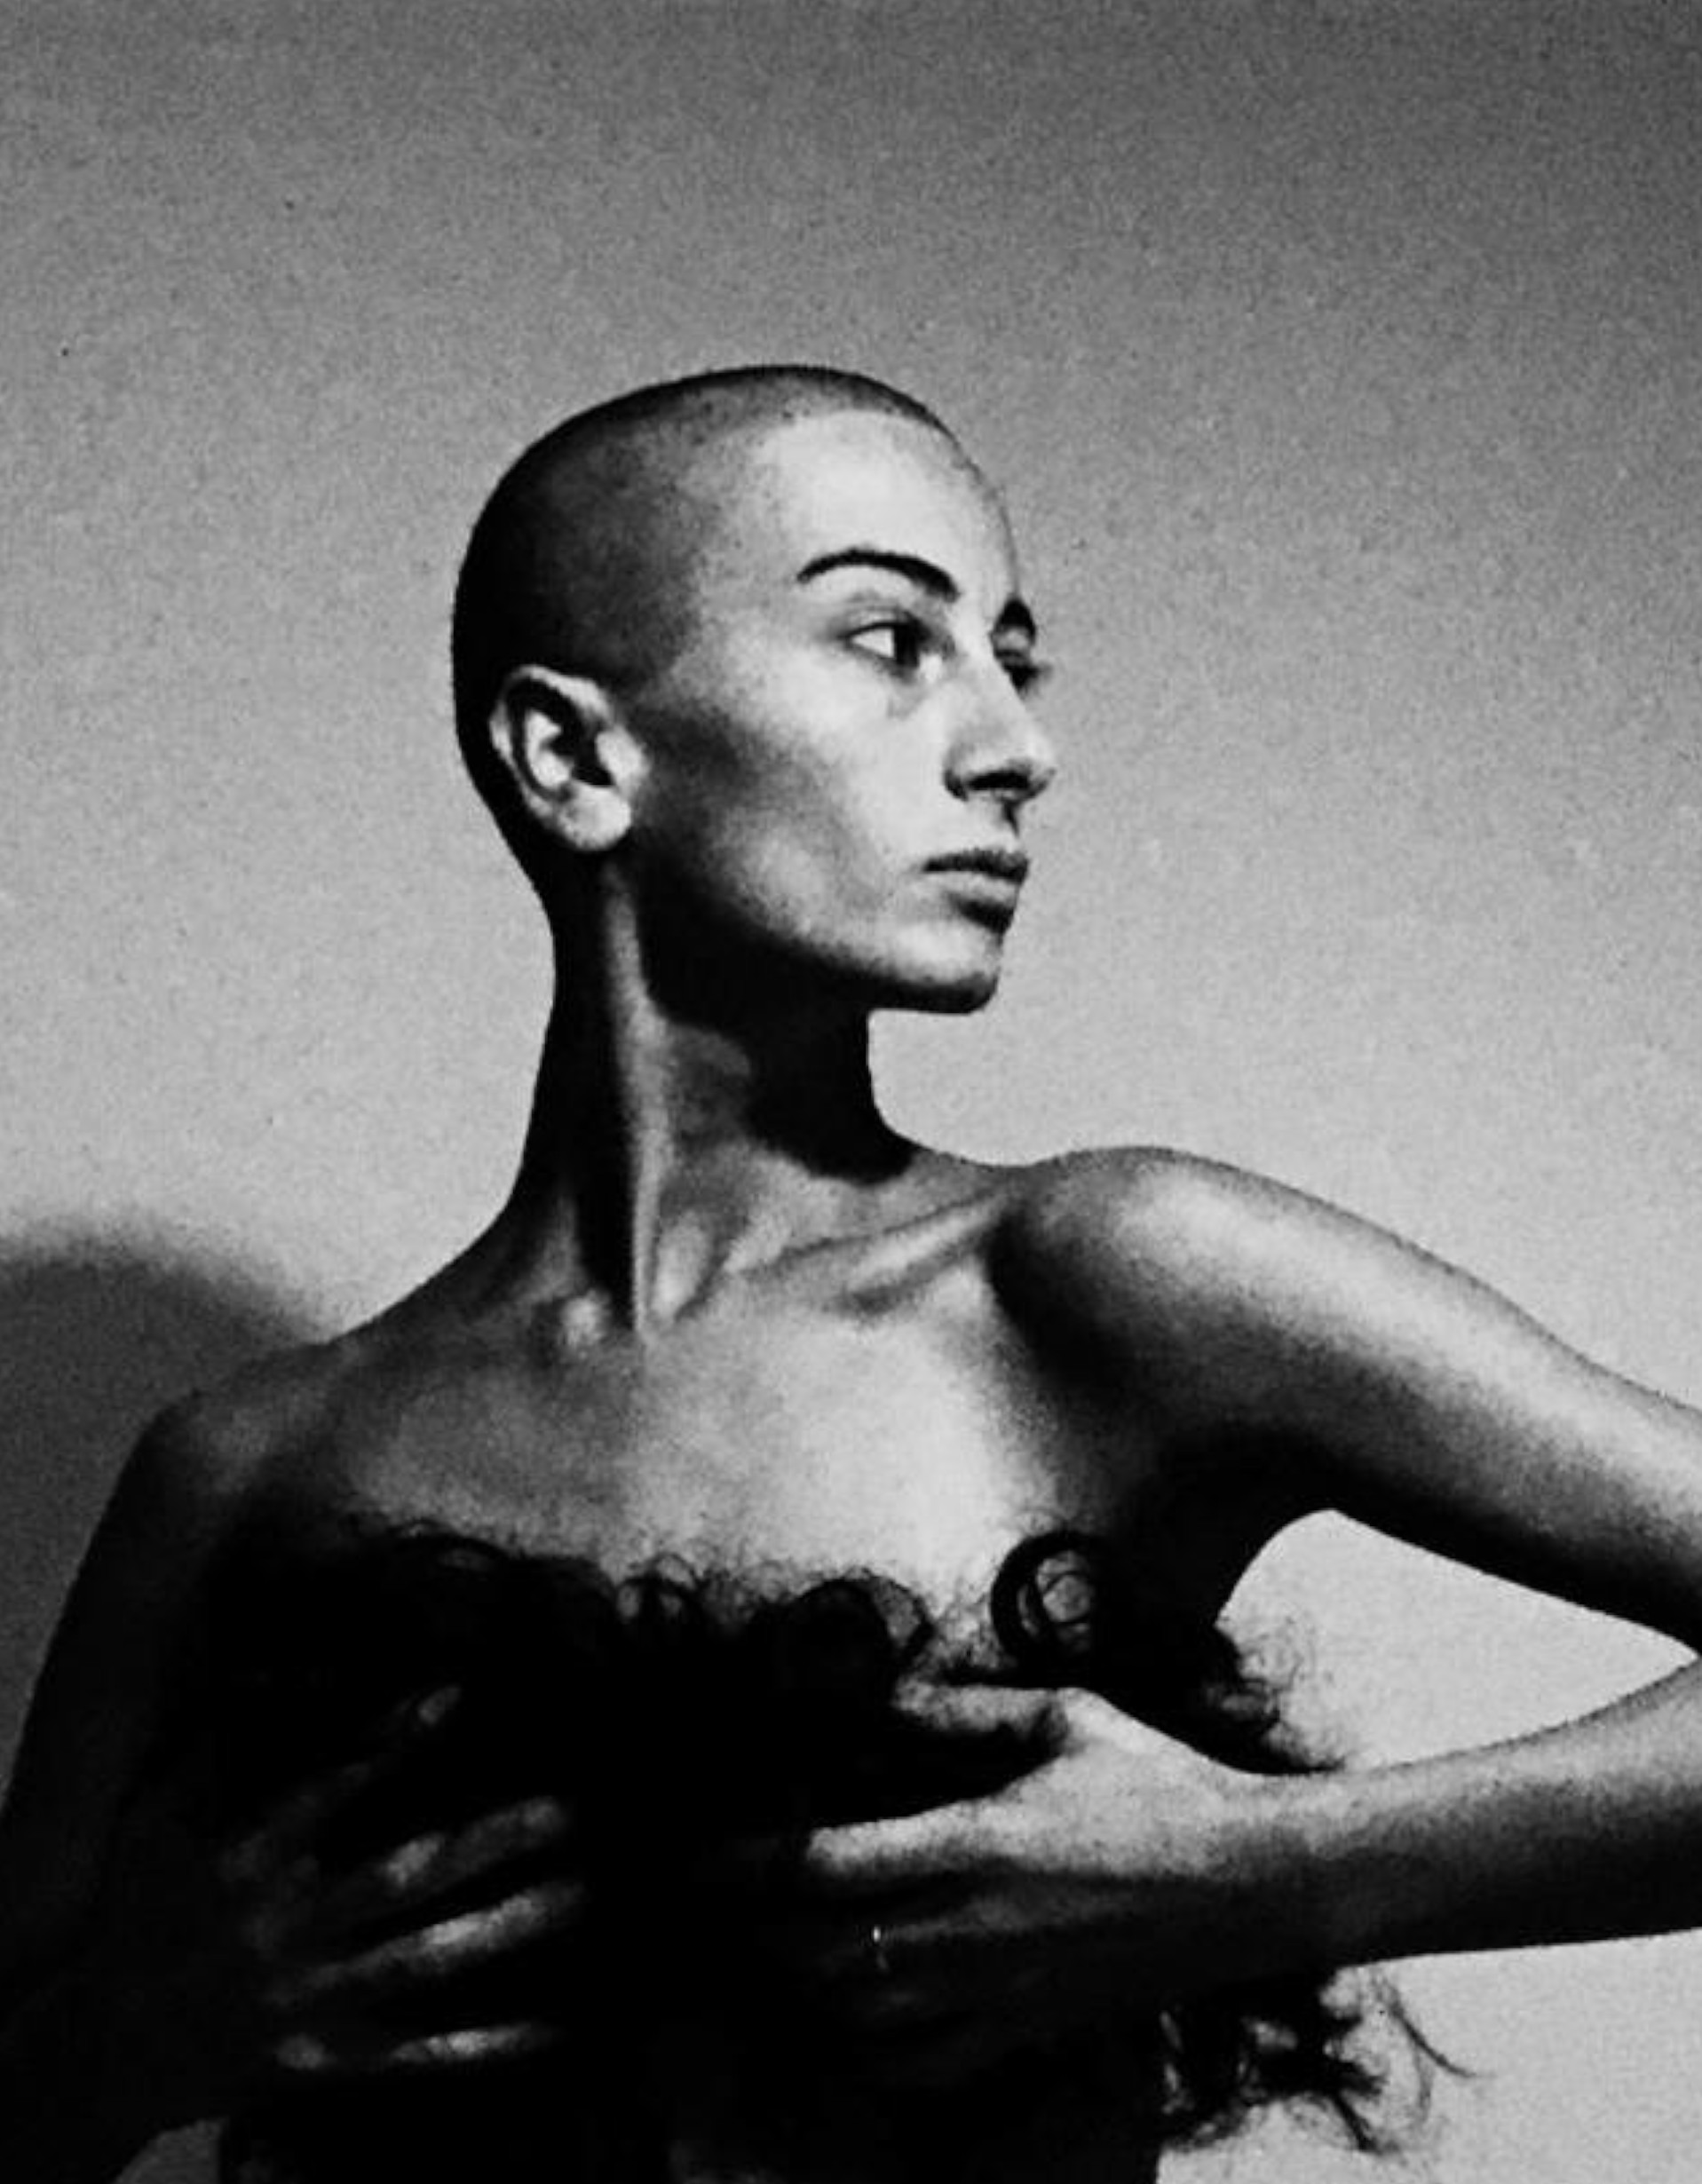
\includegraphics[width=1.1cm,left]{images/portrait}
    \vspace*{-30pt}
\end{figure}

\MyName{StephiFriedrich}
\MySlogan{Curriculum Vitae}

\sepspace

%%% ------------------------------------------------------------
\NewPart{Persoenliche Details}{}

\PersonalEntry{Geboren}{Maerz 19, 1986}
\PersonalEntry{Ort}{Düsseldorf, Germany}
\PersonalEntry{E-Mail}{\url{friedrich.stephanie@gmx.net}}
\PersonalEntry{Wohnhaft}{Krahestraße 40, 40233 Duesseldorf}

%%% ------------------------------------------------------------
\NewPart{Ausbildung}{}

\EducationEntry{Akademiebrief / Freie Malerei}{2020}{Kunstakademie Duesseldorf}{Collagehaftes bildnerisches Arbeiten mit den eigenen Mitteln}
\EducationEntry{Erste Staatsprüfung für das Lehramt an GyGe}{2018}{Gesamtnote 2,3}
\EducationEntry{Kunst auf Lehramt und freier Malerei}{WS 2007 - SS 2099}{Alanus Hochschule Alfter bei Bonn}
\EducationEntry{Magister Studium m. Hauptfach Komparatistik}{WS 2006 - SS 2007}{Universität des Saarlandes}
\sepspace

%%% ------------------------------------------------------------
\NewPart{Praxiserfahrungen}{}

\EducationEntry{Sprachaufenthalt}{2005 - 2006}{Antibes, Frankreich}
\sepspace
\EducationEntry{Betreuerin}{2007 - 2010}{Mobiler Pflegedienst Clever und Richter}
\sepspace
\EducationEntry{Dozentin}{2009}{Kunstschule Bergisch Gladbach}
\sepspace
\EducationEntry{Betreuerin}{2014}{Geschwister-Scholl Gymnasium}
\sepspace
\EducationEntry{Tutorin}{2014-2018}{Kunstakademie Duesseldorf}
\sepspace
\EducationEntry{Vertretungslehrerin Fach Kunst}{2018 - 2019}{Elly-Heuss-Knapp Gymnasium, Duisburg}
\sepspace
\EducationEntry{Vertretungslehrerin Fach Kunst}{2019 - 2020}{Gesamtschule Haan}
\sepspace
\EducationEntry{freischaffende Künstlerin}{2020}{selbstständig}
\sepspace
\EducationEntry{Kunstvermittlerin}{2021}{Museum Abteiberg, Moenchengladbach}
\sepspace

%%% ------------------------------------------------------------
\NewPart{Sonstiges}{}

\SkillsEntry{}{PKW Fuehrerschein}
\SkillsEntry{}{Camino de Santiago}

\end{document}

